\section{Posets of graph rewriting events}

\subsection{From transition systems to posets}

\begin{lemma}
  \label{lemma:pos_infl}
  Let $TS = (Q,R,E,T,I,<,\dashv)$ be a transition system and let $e,e'$ be two events in $E$. Then the following hold
  \begin{enumerate}
  \item $e<e'\implies \labl(e)\xrightarrow{+}\labl(e')$;
  \item $e\dashv e' \implies\labl(e)\xrightarrow{-}\labl(e')$.
  \end{enumerate}
\end{lemma}
\begin{proof}
  \begin{enumerate}
  \item From~\autoref{def:seq_dep} $e_1 < e_2$ implies there exists two transitions $M\overset{m_1,p_1}{\Rightarrow} M_1$ and $M_1\overset{m_2,p_2}{\Rightarrow} M_2$ that are sequential dependent. For any such pair of transitions, using~\autoref{lem:completeness_causal_pair} there exists a causal pair which in turns implies that $\labl(e)\xrightarrow{+}\labl(e')$.

  \item From~\autoref{def:inhibition} $e_1 \dashv e_2$ implies there exists transition $M\overset{m_1,p_1}{\Rightarrow} M_1$ inhibiting transition $M\overset{m_2,p_2}{\Rightarrow} M_2$. For any such pair of transitions, using~\autoref{lem:completeness_inhib_pair} there exists an inhibiting pair which in turns implies that $\labl(e)\xrightarrow{-}\labl(e')$.
  \end{enumerate}
\end{proof}

%% \begin{remark}
%%   Sequential dependence (~\autoref{def:seq_dep}) is not transitive. Therefore when considering posets in~\autoref{def:poset}, we need to distinguish between the \emph{immediate} order relation (the cover relation in~\autoref{def:poset}) and its transitive closure. %We denote the first $\cover$ and the latter with $\tleq$.
%% \end{remark}

\begin{definition}[The abstraction on a trace]
  \label{def:abstraction}
  \begin{itemize}
  \item[] $~$
  \item Let $\theta:M_0\overset{m_1,p_1}{\Rightarrow} M_1\overset{m_2,p_2}{\Rightarrow} M_2 \cdots \overset{m_n,p_n}{\Rightarrow} M_n$ be a trace. Define $\leq$ the transitive and reflexive closure of sequential dependence. We say that $\theta$ is a \emph{causal trace} if it is directed.
    %% w.r.t. the transitive closure of sequential dependence:
    %%     \[
    %%     M_i \Rightarrow M_{i+1} \tleq M_{n-1}\Rightarrow M_n, \forall i\leq n
    %%     \]
    Let us denote with $\Theta$ the set of causal traces.
  \item Define $\alpha:\Theta\to\mathcal{S}$ an \emph{abstraction} function that maps a trace into a poset as follows:
    \begin{itemize}
    \item given a transition $M\overset{m,p}{\Rightarrow} M'$ define the \emph{abstract event} $e$ associated to it
      \[
      \alpha(M\overset{m,p}{\Rightarrow} M') = e
      \]
      such that $\labl(e) = p$.
    \item define a poset from a trace $\alpha(\theta) = (E,\leq,\labl)$ such that $\alpha$ is a bijection between transitions and abstract events and such that the (the transitive and reflexive closure of) sequential dependence between transitions is preserved:
      \begin{align*}
        \alpha(t_i:M_{i-1}\overset{m_{i},p_{i}}{\Rightarrow}M_i) = e_i \\
        e_i \leq e_j \iff t_i \leq t_j \text{ and } \alpha(t_i)=e_i, \alpha(t_j)=e_j.
      \end{align*}
    \end{itemize}
  \item
    Let $TS = (Q,R,E,T,I,<,\dashv)$ be a transition system and let $\Theta = \{\theta_1,\cdots,\theta_n\}$ be a set of traces of $TS$.
    Define the set of posets $\mathcal{S}$ obtained by abstraction on $\Theta$ as follows
    \[
    \alpha(\{\theta_1,\cdots,\theta_n\}) = (s_1,\cdots, s_k)\text{ with }k\leq n
    \]
    where for each poset $s = (E,\leq,\labl)$ there exists at least one trace $\theta\in\Theta$ such that $\alpha(\theta) = (E,\leq,\labl)$.
  \end{itemize}
\end{definition}

\begin{property}
  If $\Theta$ is a set of causal traces, then all posets in $\alpha(\Theta)=\mathcal{S}$ are directed.
\end{property}

%Instead of working on the transition system, we interpret ou logic over a set of stories, $\mathcal{S}$ with the constraint that $\mathcal{S}$ is closed under set inclusion: $s\in \mathcal{S} \implies \forall s'\subset_{\labl} s, s'\in\mathcal{S}$. We equip the set of stories $\mathcal{S}$ with the binary relation $\dashv_{\mathcal{S}}$, which is the restriction of $\dashv$ to the set of events $\cup_{s\in\mathcal{S}} E_s$.

%We are not interested in the extraction mechanism, as long as the identity of events and the relationships between them (causality and inihibition) are preserved.

%In the following subsection we define the \emph{concretisation} function.

\subsection{Refinement of graph rewriting rules}

In a poset of $\mathcal{S}$, we have that for any event, its immediate causes have a positive influence on it (\autoref{lemma:pos_infl}).

\begin{definition}[Decorate posets with the positive influence]
  \begin{enumerate}
  \item[] $~$
  \item Given a set of events $E$ and a labeling function $\labl$ on events, define a function $\decor:E\times E \to E\times E\times G$ that associates to a pair of events $(e,e')$ the following set
    \[
    \decor(e,e') = \{(e,e',O) : O\text{ is a graph such that }\labl(e)\redl{+}_O \labl(e')\}.
    \]

  \item Let $s = (E,\leq,\labl)$ be a poset. A \emph{decorated} poset of $s$, denoted $s^{\star}$, is defined as follows
    \[
    s^{\star} = (E,\sqsubseteq,\labl), \text{ where }e\sqsubset_O e' \iff (e,e',O)\in\decor(e,e')\text{ and }e\cover e'.
    \]
    We denote $\decor(s)$ the set of all decorated posets of $s$.
  \end{enumerate}
\end{definition}

Let us first give an example of a refinement of a poset and then introduce all notions we need formally.
\begin{example}
\label{ex:e1e2e3}
Let us consider the poset $(\{e_1,e_2,e_3,e_4\},\sqsubset)$ where $e_1\sqsubset_{O_1}e_2\sqsubset_{O_2}e_3$, $e_4\sqsubset_{O_4}e_3$ and $\labl(e_1)=r_1$, $\labl(e_2)=r_2$, $\labl(e_3)=r_3$, $\labl(e_4)=r_4$.

First we refine $r_2$ using the relation $r_1\redl{+}_{O_1} r_2$, (as we have seen in~\autoref{def:low_res}):
\[
\begin{tikzpicture} %[scale=0.8]
  \node (o1) at (0,-1) {\(O_1\)};
  \node (m1) at (0,1) {\(M_1\)};
  \node (n1) at (2,1) {\(N_1\)};
  \node (r1) at (-1,0) {\(R_1\)};
  \node (l1) at (-2.5,0) {\(L_1\)};
  \node (l2) at (1,0) {\(L_2\)};
  \node (r2) at (2.5,0) {\(R_2\)};
  \draw [->] (o1) -- (r1);
  \draw [->] (o1) -- (l2);
  \draw [->] (r1) -- (m1);
  \draw [->] (r2) -- (n1);
  \draw [->] (l2) -- (m1);
  \draw [vecArrow] (l1) -- (r1);
  \draw [vecArrow] (m1) -- (n1);
  \draw [vecArrow] (l2) -- (r2);
\end{tikzpicture}
\]
We apply a rewriting step to $M_1$ using rule $r_2$ to obtain $N_2$. We refine then $r_3$ using $N_2$ (this step is formally defined in~\autoref{def:seq_comb}):
\[
\begin{tikzpicture} %[scale=0.8]
  \node (o1) at (0,-1) {\(O_1\)};
  \node (m1) at (0,1) {\(M_1\)};
  \node (r1) at (-1,0) {\(R_1\)};
  \node (l1) at (-2.5,0) {\(L_1\)};
  \node (l2) at (1,0) {\(L_2\)};
  \node (r2) at (2.5,0) {\(R_2\)};
  \node (o2) at (3.5,-1) {\(O_2\)};
  \node (l3) at (4.5,0) {\(L_3\)};
  \node (r3) at (6,0) {\(R_3\)};
  \node (m2p) at (2.5,1) {\(N_1\)};
  \node (n) at (3.5,2) {\(M_2\)};
  \node (n2) at (5,2) {\(N_2\)};
  \draw [->] (o1) -- (r1);
  \draw [->] (o1) -- (l2);
  \draw [->] (r1) -- (m1);
  \draw [->] (l2) -- (m1);
  \draw [->] (o2) -- (r2);
  \draw [->] (o2) -- (l3);
  \draw [->] (l3) -- (n);
  \draw [->] (m2p) -- (n);
  \draw [->] (r2) -- (m2p);
  \draw [->] (r3) -- (n2);
  \draw [vecArrow] (l1) -- (r1);
  \draw [vecArrow] (l2) -- (r2);
  \draw [vecArrow] (l3) -- (r3);
  \draw [vecArrow] (m1) -- (m2p);
  \draw [vecArrow] (n) -- (n2);
\end{tikzpicture}
\]
Let us now integrate $e_4\sqsubset_{O_4} e_3$ in the sequence. Let $R_4\lemb M_3\remb L_3$ be the cospan obtained from $\labl(e_4)\redl{+}_O\labl(e_3)$.
We combine $M_2$ and $M_3$ using $L_3$ (concurrent combinator is formally introduced in~\autoref{def:conc_comb}):
\[
\begin{tikzpicture} %[scale=0.8]
  \node (l4) at (0.5,0) {\(L_4\)};
  \node (r4) at (2,0) {\(R_4\)};
  \node (o4) at (3,-1) {\(O_4\)};
  \node (m4) at (3,1) {\(M_3\)};
  \node (l3) at (4,0) {\(L_3\)};
  \node (r3) at (5.5,0) {\(R_3\)};
  \node (m2p) at (5,1) {\(M_2\)};
  \node (n) at (4,2) {\(M_4\)};
  \draw [->] (o4) -- (r4);
  \draw [->] (o4) -- (l3);
  \draw [->] (r4) -- (m4);
  \draw [->] (l3) -- (m4);
  \draw [->] (m4) -- (n);
  \draw [->] (m2p) -- (n);
  \draw [->] (l3) -- (m2p);
  \draw [vecArrow] (l4) -- (r4);
  \draw [vecArrow] (l3) -- (r3);
\end{tikzpicture}
\]
The refinement of our poset is then the following set of transitions:
\[
\begin{tikzpicture} %[scale=0.8]
  \node (o1) at (0,-1) {\(O_1\)};
  \node (m1) at (0,1) {\(M_1\)};
  \node (r1) at (-1,0) {\(R_1\)};
  \node (l1) at (-2.5,0) {\(L_1\)};
  \node (l2) at (1,0) {\(L_2\)};
  \node (r2) at (2.5,0) {\(R_2\)};
  \node (o2) at (3.5,-1) {\(O_2\)};
  \node (l3) at (4.5,0) {\(L_3\)};
  \node (r3) at (6,0) {\(R_3\)};
  \node (n1) at (2.5,1) {\(N_1\)};
  \node (m2) at (3.5,2) {\(M_2\)};
  \node (m4) at (3.5,3) {\(M_4\)};
  \node (n4) at (6,3) {\(N_4\)};
  \draw [->] (o1) -- (r1);
  \draw [->] (o1) -- (l2);
  \draw [->] (r1) -- (m1);
  \draw [->] (l2) -- (m1);
  \draw [->] (o2) -- (r2);
  \draw [->] (o2) -- (l3);
  \draw [->] (l3) -- (m2);
  \draw [->] (n1) -- (m2);
  \draw [->] (r2) -- (n1);
  \draw [->] (r3) -- (n4);
  \draw [vecArrow] (l1) -- (r1);
  \draw [vecArrow] (l2) -- (r2);
  \draw [vecArrow] (l3) -- (r3);
  \draw [vecArrow] (m1) -- (n1);
  \draw [->] (m2) -- (m4);
  \draw [vecArrow] (m4) -- (n4);
\end{tikzpicture}
\]

%% Lastly we have to propagate $M_4$ backwards to events $e_1$, $e_2$ and $e_4$.
%% \[
%% \begin{tikzpicture} %[scale=0.8]
%%   \node (o1) at (0,-1) {\(O_1\)};
%%   \node (m1) at (0,1) {\(M_1\)};
%%   \node (r1) at (-1,0) {\(R_1\)};
%%   \node (l1) at (-2.5,0) {\(L_1\)};
%%   \node (l2) at (1,0) {\(L_2\)};
%%   \node (r2) at (2.5,0) {\(R_2\)};
%%   \node (o2) at (3.5,-1) {\(O_2\)};
%%   \node (l3) at (4.5,0) {\(L_3\)};
%%   \node (r3) at (6,0) {\(R_3\)};
%%   \node (n1) at (2.5,1) {\(N_1\)};
%%   \node (m2) at (3.5,2) {\(M_2\)};
%%   \node (n2) at (6,2) {\(N_2\)};
%%   \node (m6) at (-2.5,3) {\(M_6\)};
%%   \node (m5) at (0,3) {\(M_5\)};
%%   \node (m4) at (3.5,3) {\(M_4\)};
%%   \node (n4) at (6,3) {\(N_4\)};
%%   \draw [->] (o1) -- (r1);
%%   \draw [->] (o1) -- (l2);
%%   \draw [->] (r1) -- (m1);
%%   \draw [->] (l2) -- (m1);
%%   \draw [->] (o2) -- (r2);
%%   \draw [->] (o2) -- (l3);
%%   \draw [->] (l3) -- (m2);
%%   \draw [->] (n1) -- (m2);
%%   \draw [->] (r2) -- (n1);
%%   \draw [->] (r3) -- (n2);
%%   \draw [vecArrow] (l1) -- (r1);
%%   \draw [vecArrow] (l2) -- (r2);
%%   \draw [vecArrow] (l3) -- (r3);
%%   \draw [vecArrow] (m1) -- (n1);
%%   \draw [vecArrow] (m2) -- (n2);
%%   \draw [->] (n2) -- (n4);
%%   \draw [->] (m2) -- (m4);
%%   \draw [->] (m1) -- (m5);
%%   \draw [->] (l1) -- (m6);
%%   \draw [vecArrow] (m4) -- (n4);
%%   \draw [vecArrow] (m4) -- (m5);
%%   \draw [vecArrow] (m5) -- (m6);
%% \end{tikzpicture}
%% \]
%% The refinement of our poset is then the set of transitions
%% \[
%% \begin{tikzpicture} %[scale=0.8]
%%   \node (m6) at (0,1) {\(M_6\)};
%%   \node (m5) at (1.5,1) {\(M_5\)};
%%   \node (m4) at (3,1) {\(M_4\)};
%%   \node (n4) at (4.5,1) {\(N_4\)};
%%   \node (m7) at (1.5,0) {\(M_7\)};
%%   \draw [vecArrow] (m4) -- (n4);
%%   \draw [vecArrow] (m5) -- (m4);
%%   \draw [vecArrow] (m6) -- (m5);
%%   \draw [vecArrow] (m7) -- (m4);
%% \end{tikzpicture}
%% \]
%% where $M_7$ is obtained by a rewriting of $M_4$ using rule $r_4$.
\end{example}

\begin{definition}[Refinement of a rule~\cite{information_carriers}]
  Let $r:L{\Rightarrow} R$ be a rule and let $m:L\emb M$ be a matching in a graph $M$. The production $M\overset{m,r}{\Rightarrow} N$ obtained by DPO rewriting of $M$ using the rule $r$ is called a \emph{refinement} of $r$.
\end{definition}

\begin{definition}[Refinement of a poset]
  \label{def:ref_poset}
  Given a poset $s=(E,<,\labl)$ of graph rewriting events, the \emph{refinement} of $s$, is a bijection $\imath$ between events $e\in E$ and transitions $M\overset{m,p}{\Rightarrow} M'$ such that
  \begin{itemize}
  \item the label of an event is rule in the transition: $\labl(e)=p$;
  \item for all $e_1,e_2\in E$, if $e_1<e_2$ and $\imath(e_1) = M_1\overset{m_1,p_1}{\Rightarrow} M_1'$, $\imath(e_2) =M_2\overset{m_2,p_2}{\Rightarrow} M_2'$ then $M_1'\emb M_2$.
  \end{itemize}
\end{definition}

%Before giving the construction of a refinement $(M_i\overset{m_i,p_i}{\Rightarrow} M_{i+1})_{e_i\in E}$ let us first introduce some combinators of contexts.

%% \begin{definition}[Propagate a context]
%%   \label{def:propagate}
%%   Given a sequence $M_1{\Rightarrow} M_2\cdots {\Rightarrow} M_n\cdots {\Rightarrow} M_{m}$ and a graph $M_{n}'$ with $M_n\emb M_{n}'$ define the \emph{propagation} of $M_{n}'$ as the sequence  $M_1'{\Rightarrow} M_2'\cdots {\Rightarrow} M_n'\cdots {\Rightarrow} M_{m}'$ where
%%   \begin{itemize}
%%   \item $M_i'$, for $i<n$, is obtained by the reverse of the production $M_i\Rightarrow M_{i+1}$ applied to the new contexts;
%%   \item $M_i'$, for $n<i\leq m$, is obtained by the production $M_i\Rightarrow M_{i+1}$ applied to the new contexts.
%%   \end{itemize}
%% \end{definition}

\begin{definition}[Sequential combinator]
\label{def:seq_comb}
  Let $M\Rightarrow N$ and $L\Rightarrow R$ be two productions such that there exists $N\remb O \lemb L$ a cospan.
  Define the sequential combinator as follows:
  \[
  (M\overset{m,p}{\Rightarrow}N)\oplus_O (L\Rightarrow R) = M'\overset{m',p'}{\Rightarrow}N'
  \]
  where $N\emb M' \remb L$ is the pushout of the cospan $N\remb O \lemb L$ and $N'$ is obtained by a DPO rewriting of $M'$ by the production $L\Rightarrow R$:
  \[
  \begin{tikzpicture} %[scale=0.8]
    \node (o) at (0,-1) {\(O\)};
    \node (mp) at (0,1) {\(M'\)};
    \node (m) at (-2.5,0) {\(M\)};
    \node (n) at (-1,0) {\(N\)};
    \node (l) at (1,0) {\(L\)};
    \node (r) at (2.5,0) {\(R\)};
    \node (np) at (2,1) {\(N'\)};
    \draw [->] (o) -- (n);
    \draw [->] (o) -- (l);
    \draw [->] (n) -- (mp);
    \draw [->] (l) -- (mp);
    \draw [->] (r) -- (np);
    \draw [vecArrow] (m) -- (n);
    \draw [vecArrow] (l) -- (r);
    \draw [vecArrow] (mp) -- (np);
  \end{tikzpicture}
  \]
  We denote $m'$ the morphism $L\to M'$ and $p'$ the production $L\Rightarrow R$.
\end{definition}

\begin{definition}[Wide pushout~\cite{wide}]
The wide pushout of a family of morphisms $(P\to M_i)_i$ consists of a graph $M$ and a family of morphisms $(M_i\to M)_i$ such that the diagram commutes
\[
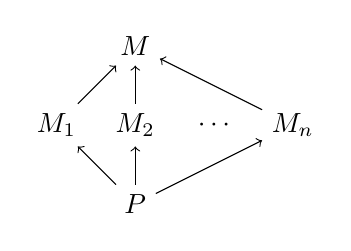
\begin{tikzpicture} %[scale=0.8]
  \node (o) at (0,-1) {\(P\)};
  \node (m1) at (-1,0) {\(M_1\)};
  \node (m2) at (0,0) {\(M_2\)};
  \node (text) at (1,0) {\(\cdots\)};
  \node (mn) at (2,0) {\(M_n\)};
  \node (m) at (0,1) {\(M\)};
  \draw [->] (o) --  (m1);
  \draw [->] (o) --  (m2);
  \draw [->] (o) --  (mn);
  \draw [->] (m1) --  (m);
  \draw [->] (m2) --  (m);
  \draw [->] (mn) --  (m);
\end{tikzpicture}
\]
for any other $M'$ and family of morphisms $(M_i\to M')_i$ there exists a unique morphism $M\to M'$ that commutes.

The wide pushout is equivalent to computing the pushout pairwise on $(P\to M_i)_i$.
\end{definition}

\begin{lemma}[Concurrent combinator]
  \label{def:conc_comb}
  Let $(M_i)_{0< i< n}$ be a family of graphs, let $(M'\emb M_i)_{0< i< n}$ be a family of injective morphisms and let $p:L\Rightarrow R$ be a production.
  Define the concurrent combinator as follows:
  \[
  \otimes_{L{\Rightarrow}R}(M_1, M_2,\cdots M_n) = M \overset{m,p}{\Rightarrow} N
  \]
  where $M$ is the wide pushout of the family of morphisms $(L\emb M_i)_i$.

  The morphisms $m_i$, obtained by the composition of $L\emb M_i$ and $M_i\emb M$ are equivalent. We denote $m$ one such morphism.

  The graph $N$ is obtained by a DPO rewriting of $M$ by the production $p$.
\end{lemma}
\begin{proof}
  First we prove that the morphisms $m_i$ obtained by the composition of $M'\emb M_i$  and $M_i\emb M$ are equivalent.
% which follows from the definition of the pushout.
  Secondly we show that the gluing conditions hold for the DPO rewriting of $p$ on $M$ iff they hold for the dpo rewriting of $p$ on all $M_i$. Both follow from $(M_i\to M)_i$ being the wide pushout of $(L\to M_i)_i$.
\end{proof}

\begin{definition}[Refinement propagation]
  \label{def:ref_propagator}
  Let $s=(E,\tleq,\labl)$ be a poset and let $(E,\sqsubset,\labl)\in \decor(s)$ be a decoration of $s$.
  We define a function, called the \emph{forward propagator}, by induction on $s$:
  \begin{align*}
    &\fp(e) = L\Rightarrow R&\text{ if }e\in\text{min}(s)\text{ and }\labl(e) = L\action R\\
    &\fp(e) = M\overset{m,p}{\Rightarrow} N&\text{ where }\forall e_i, e_i\sqsubset_{O_i}e,
    \fp(e_i)\oplus_{O_i}L\Rightarrow R= M_i\overset{m_i,p}{\Rightarrow} N_i\\
    &&\otimes_{\labl(e)}(M_1, M_2, \cdots M_n) = M \overset{m,p}{\Rightarrow} N
    \text{and }\labl(e) = p:L\action R\\
  \end{align*}
\end{definition}

\begin{lemma}
  $(E,\sqsubset,\labl,\fp)$ is a refinement of $(E,<,\labl)$.
\end{lemma}
\begin{proof}
  For the base case we have only to show that, for $\fp(e) = M\overset{m,p}{\Rightarrow} N$, $\labl(e)=p$. This follows from~\autoref{def:seq_comb} and~\autoref{def:conc_comb}.

  For the inductive case, let us consider an event $e$. As above, we have that if $\fp(e) = M\overset{m,p}{\Rightarrow} N$ then $\labl(e)=p$. If there exists $e'$, $e'\sqsubset_O e$ with $\fp(e')= M'\overset{m',p'}{\Rightarrow} N'$ then, from~\autoref{def:ref_propagator} and from~\autoref{def:seq_comb}, there exists $M''$ such that $M'\emb M''$. Moreover, from~\autoref{def:conc_comb}, $M''\emb M$.
\end{proof}

%% \begin{definition}[Refinement propagation]
%%   \label{def:ref_propagator}
%%   Let us define two functions the forward propagator $\fp$, and the backward propagator $\bp$, that map events in a poset $\{E,\sqsubset,\labl\}$ to transitions.
%% We proceed by induction on the transitive and reflexive closure of the cover relation $\sqsubset$ and start with the minimal events for the definition of $\fp$. For the definition of $\bp$ we proceed by induction on the transitive and reflexive closure of the reverse relation $\sqsubset^{-1}$ starting with the maximal events for $\bp$:
%% \begin{align*}
%%   \text{forward propagator}\\
%%   &\fp(e) = \labl(e)&\text{ if }e\in\text{min}(s)\\
%%   &\fp(e) = M\Rightarrow N&\text{ where }\forall e_i, e_i\sqsubset_{O_i}e, \fp(e_i)\oplus_{O_i}\labl(e) = M_i\Rightarrow N_i\\
%%   &&\otimes_{\labl(e)}(M_1, M_2, \cdots M_n) = M \Rightarrow N\\
%%   \\
%%   \text{backward propagator}\\
%%   &\bp(e) = \fp(e)&\text{ if }e\in\text{max}(s)\\
%%   &\bp(e) = M\Rightarrow N&\text{ where }\forall e_i, e\sqsubset_{O_i}e_i, \bp(e_i) = M_i\Rightarrow N_i\\
%%   &&\otimes_{\fp(e)^{-1}}(M_1, M_2, \cdots M_n) = M \Rightarrow N
%% \end{align*}
%% \end{definition}

%% \begin{definition}[Embeddings between transitions]
%%   A transition $M'\overset{m',p}\Rightarrow N'$ embeds into a transition $M\overset{m,p}\Rightarrow N$ if there exists a morphism $h:M'\to M$ such that the diagram commutes:
%%   \[
%%   \begin{tikzpicture} %[scale=0.8]
%%     \node (d) at (0,2.5) {\(D\)};
%%     \node (m) at (-2,2.5) {\(M\)};
%%     \node (n) at (2,2.5) {\(N\)};
%%     \node (m1) at (-2,1) {\(M'\)};
%%     \node (d1) at (0,1) {\(D'\)};
%%     \node (n1) at (2,1) {\(N'\)};
%%     \node (l) at (-2,-0.5) {\(L\)};
%%     \node (k) at (0,-0.5) {\(K\)};
%%     \node (r) at (2,-0.5) {\(R\)};
%%     \draw [left hook->] (l) -- node [right,midway] {$m'$} (m1);
%%     \draw [left hook->] (r) -- (n1);
%%     \draw [left hook->] (k) -- (d1);
%%     \draw [left hook->] (k) -- (l);
%%     \draw [left hook->] (k) -- (r);
%%     \draw [dotted, left hook->] (m1) -- (m);
%%     \draw [dotted, left hook->] (d1) -- (d);
%%     \draw [dotted, left hook->] (n1) -- (n);
%%     \draw [left hook->] (d1) -- (m1);
%%     \draw [left hook->] (d1) -- (n1);
%%     \draw [left hook->] (d) -- (m);
%%     \draw [left hook->] (d) -- (n);
%%     \draw [left hook->] (l) to [bend left] node [left,midway] {$m$} (m);
%%     \draw [left hook->] (k) to [bend right] (d);
%%     \draw [left hook->] (r) to [bend right] (n);
%%   \end{tikzpicture}
%%   \]
%% \end{definition}

%% \begin{lemma}
%%   \label{lem:subposet}
%%   Let $s'\subseteq s$ be a connected poset (i.e. directed either upwards or downwards). Then
%%   \[\forall e\in s', \bp_{s'}(e)\text{ embeds into }\bp_s(e),\]
%%   where $\bp_s(e)$ is the refinement of~\autoref{def:ref_propagator} applied to $s$.
%%   A \textbf{corollary} is that if two transitions are sequential dependent in $\bp_{s'}$ then they are sequential dependent in $\bp_{s}$.
%% \end{lemma}
%% \begin{proof}
%%   \begin{mdframed}[backgroundcolor=blue!20]
%%     to do
%%   \end{mdframed}
%% \end{proof}


%% \begin{example}[Feedback loops]
%% Let us show how we can interpret negative feedback loops. Let $e_1\in s_1\redl{-} e_2\in s_2$ such that $s_2\subset s_1$. Then $e_2\leq_{s_1} e_2$. However this additional constraint does not change the way we interpret negative influence, that is the influence is realised if there exists $M$ such that the following diagram commutes:
%% \[
%% \begin{tikzpicture} %[scale=0.8]
%%   \node (o) at (0,0) {\(O\)};
%%   \node (n) at (0,2) {\(M\)};
%%   \node (l1) at (-1,0) {\(L_1\)};
%%   \node (l2) at (1,0) {\(L_2\)};
%%   \node (n1) at (-1,1) {\(M_1\)};
%%   \node (n2) at (1,1) {\(M_2\)};
%%   \draw [->] (l1) -- (n1);
%%   \draw [->] (l2) -- (n2);
%%   \draw [->] (o) -- (n1);
%%   \draw [->] (o) -- (n2);
%%   \draw [->] (n1) -- (n);
%%   \draw [->] (n2) -- (n);
%% \end{tikzpicture}
%% \]
%% \end{example}


\subsection{Interpreting inhibition on posets}

In interpreting our logic, we work with a set of posets in $\mathcal{S}$ and a set of events $\cup_{s\in\mathcal{S}} E_s$.

\begin{definition}[Refinement of an event in a poset]
  Let $e$ be an event in a poset $s=\{E,<,\labl\}$.
  Define $\mathcal{R}(e\in s) = M\Rightarrow N$ where $\{E,<,\labl,\imath\}$ is a refinement of $s$ and $\imath(e) = M\Rightarrow N$.
  %We call such a graph $M$ a \emph{context of application} of $e$ in $s$.
\end{definition}

\begin{definition}[Refinement based on negative influence]
\label{def:ref_neg_infl}
  For two posets $s_1,s_2$ and two events $e_1\in s_1$ and $e_2\in s_2$ let the following be their refinements $\mathcal{R}(e_1\in s_1) = M_1\Rightarrow N_1$ and $\mathcal{R}(e_2\in s_2) = M_2\Rightarrow N_2$. Define $\mathcal{R}(e_1\in s_1\redl{-} e_2\in s_2) = M$ for which the diagram below commutes:
  \[
  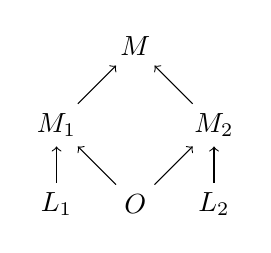
\begin{tikzpicture} %[scale=0.8]
    \node (o) at (0,0) {\(O\)};
    \node (n) at (0,2) {\(M\)};
    \node (l1) at (-1,0) {\(L_1\)};
    \node (l2) at (1,0) {\(L_2\)};
    \node (n1) at (-1,1) {\(M_1\)};
    \node (n2) at (1,1) {\(M_2\)};
    \draw [->] (l1) -- (n1);
    \draw [->] (l2) -- (n2);
    \draw [->] (o) -- (n1);
    \draw [->] (o) -- (n2);
    \draw [->] (n1) -- (n);
    \draw [->] (n2) -- (n);
  \end{tikzpicture}
  \]
  where $\labl(e_1)\redl{-}_O\labl(e_2)$, for some graph $O$.
\end{definition}

\subsection{From posets to traces}

\begin{definition}[Linear extensions of posets]
  A linear extension, denoted $\underline{s}$, of a poset $s=(E,\tleq)$ is any total order that extends the partial order $\tleq$. We denote $\linear(s)$ the set of all possible linear extensions of $s$.
  \[
  (E,\seq)\in\linear(s) \iff \forall e_1,e_2\in E, e_1\leq e_2\implies e_1\seq e_2.
  \]
\end{definition}

\begin{lemma}
  \label{lemm:linear_to_trace}
  Let $s=(E,\leq,\labl)$ be a directed poset, with $s^{\star}\in\decor(s)$ one of its decorations and with $\underline{s^{\star}}\in\linear(s^{\star})$ a linear extension of $s^{\star}$. Moreover, let $(E,\leq,\labl,\fp)$ the refinement of $s^{\star}$.

  There is a function, denoted $\bp$, that converts $\underline{s^{\star}}$ into a trace such that
  \[
  \forall \theta\in \Theta, \exists \theta'\in\bp(\linear(\decor(\alpha(\Theta))))\text{ s.t. } \theta'\text{ embeds in }\theta.
  \]
\end{lemma}
\begin{proof}

  Let us first define the function $\bp$, called the \emph{backward propagator}, by induction on the reverse order in $\underline{s^{\star}}$.
  If $e_1\in\text{max}(\underline{s^{\star}})$, then $\bp(e_1) = \fp(e_1)$.
  Otherwise, for $e_1\in\underline{s^{\star}}$, we have that $e_1\prec e_2\prec\cdots e_n$ and $e_2,.., e_n$ are the events for which $\bp$ is defined so far.

  Let $e_2,e_k\in\underline{s^{\star}}$ be two events such that
  \begin{align}
    &e_1\prec e_2\text{ and there is no }e_2'\text{ with } e_1\prec e_2'\prec e_2\\
    \label{eq:e3}
    &e_1\sqsubset_O e_k\text{ and there is no }e_k'\neq e_k\text{ with } e_1\preceq e_k'\preceq e_k, 2\leq k\leq n.
  \end{align}
  As both events precede $e_1$ in $\underline{s^{\star}}$, we have that
  \begin{align}
    \bp(e_2) = M_2\Rightarrow N_2 \text{ and } \bp(e_k) = M_k\Rightarrow N_k.
  \end{align}
  Also, from the properties of refinement (\autoref{def:ref_poset}), we have that there exists a morphism $h$ such that
  \begin{align}
    \label{eq:matching}
    \fp(e_k)=M_k'\Rightarrow N_k', \fp(e_1)=M_1'\Rightarrow N_1'\text{ and }h:(M_k'\emb M_k)\circ(N_1'\emb M_k').
  \end{align}
  Next, we apply a DPO rewriting step to $M_k$ using the production $(M_1'\Rightarrow N_1')^{-1}$ and the matching $h$:
  \[
  \begin{tikzpicture} %[scale=0.8]
    \node (p1) at (0,1) {\(P_1\)};
    \node (m3) at (2,1) {\(M_k\)};
    \node (m1) at (0,0) {\(M_1\)};
    \node (n1) at (2,0) {\(N_1\)};
    \draw [->] (m1) -- (p1);
    \draw [->] (n1) -- (m3);
    \draw [vecArrow] (m3) -- (p1);
    \draw [vecArrow] (n1) -- (m1);
  \end{tikzpicture}
  \]
  \begin{mdframed}[backgroundcolor=blue!20]
    We have to show in the construction above that matching $h$ defined in~\autoref{eq:matching} allows the dpo rewriting step of $M_k$, that is that the gluing conditions hold.
  \end{mdframed}

  So far, we have a trace $M_2\Rightarrow N_2\cdots M_k\Rightarrow N_2\cdots M_n\Rightarrow N_n$ corresponding to the chain $e_2\prec e'\cdots e_k\prec e''\prec\cdots e_n$ and a transition $P_1\Rightarrow M_k$. The last step consists in "swaping" the transition $P_1\Rightarrow M_k$ at the beginning of the trace, to obtain a trace $M_1\Rightarrow M_2\Rightarrow N_2\cdots M_n\Rightarrow N_n$.

  We proceed by induction on the trace $M_2\Rightarrow N_2\cdots M_k\Rightarrow N_2\cdots M_n\Rightarrow N_n$.
  Let us consider one step of swapping: let $M_j\overset{e_j}{\Rightarrow} M_{j+1}$ and $P_j\overset{e_1}{\Rightarrow}M_{j+1}$ where $2\leq j\leq k-1$. We consider the following cases:

  \begin{itemize}
  \item {\bf both events have a common successor $\mathbf{e_j\sqsubset e_{j+1}}$ and $\mathbf{e_1\sqsubset e_{j+1}}$.} Note that from~\autoref{eq:e3} this case is only possible if $j+1=k$.

  \item {\bf events have different successors $\mathbf{e_j\sqsubset e_i}$ with $\mathbf{i\neq k}$.}
    We can rewrite the transitions $M_j\overset{e_j}{\Rightarrow} M_{j+1}\overset{e_1^{-1}}{\Rightarrow} P_j$, as productions are reversible. We distinguish again between two cases. In the diagram below:
    \[
    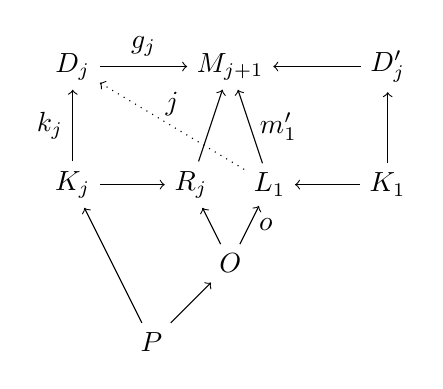
\begin{tikzpicture} %[scale=0.8]
    \node (r1) at (1.5,0) {\(R_j\)};
    \node (m1) at (2,1.5) {\(M_{j+1}\)};
    \node (l2) at (2.5,0) {\(L_1\)};
    \node (d1) at (0,1.5) {\(D_j\)};
    \node (k1) at (0,0) {\(K_j\)};
    \node (d2) at (4,1.5) {\(D_j'\)};
    \node (k2) at (4,0) {\(K_1\)};
    \node (o) at (2,-1) {\(O\)};
    \node (p) at (1,-2) {\(P\)};
    \draw [->] (k1) -- (r1);
    \draw [->] (k2) -- (l2);
    \draw [->] (k1) -- node [left,midway] {\(k_j\)} (d1);
    \draw [->] (k2) -- (d2);
    \draw [->] (d1) -- node [above,midway] {\(g_j\)} (m1);
    \draw [->] (d2) -- (m1);
    \draw [->] (l2) -- node [right,midway] {\(m_1'\)} (m1);
    \draw [->] (r1) -- (m1);
    \draw [dotted,->] (l2) -- node [above,midway] {\(j\)} (d1);
    \draw [->] (p) -- (k1);
    \draw [->] (p) -- (o);
    \draw [->] (o) -- (r1);
    \draw [->] (o) -- node [right,midway] {$o$} (l2);
    \end{tikzpicture}
    \]
    first suppose that there is a morphism $j:R_1\to D_j$ such that the diagram commutes. Then we can rewrite $M_j$ using the production of $e_1^{-1}$ and obtain the transition $M_j\overset{e_1^{-1}}{\Rightarrow}P_{j+1}$. We reverse it again and obtain $P_{j+1}\overset{e_1}{\Rightarrow} M_j$. Then the induction continues with the transitions $M_{j-1}\overset{e_{j-1}}{\Rightarrow} M_{j}$ and $P_{j+1}\overset{e_1}{\Rightarrow} M_j$.

    The second case is when there is no such morphism. We will show that this case is not possible. To do this we have to reason by induction

    If there is no morphism $j$ then there exists $O$ the pullback of $R_j\lemb M_{j+1}\remb L_1$ and $P$ the pullback of $K_j\lemb R_j\remb O$ such that the morphism $P\to O$ is not an iso.

    We also have the transition $M_{j+1}\overset{e_{j+1}}{\Rightarrow} M_{j+2}$. If




  \end{itemize}


  The construction of~\autoref{lemm:linear_to_trace} is minimal w.r.t. the choice of decoration and linear extension, in the sense that each graph in the construction is the result of a pushout.



\end{proof}




\newpage

\begin{lemma}[Refinement of a poset for trace reconstruction]
  \label{lem:rewrite_concurrent}
  Let $s=(E,\tleq,\labl)$ be a poset and
  %let $(E,\sqsubset,\labl)\in \decor(s)$ be a decoration of $s$ and
  let $(E,\sqsubset,\labl,\fp)$ be a refinement of $s$.

  Let $e_1,e_2\in E$ be two incomparable events such that
  $\fp(e_1) = M_1\overset{m_1,p_1}{\Rightarrow} M_1'$ and $\fp(e_2) = M_2\overset{m_2,p_2}{\Rightarrow} M_2'$.

  We have the following additional contraint on the refinement of $s$:
  \begin{enumerate}
  \item if the two productions are co-initial, i.e. $M_1\iso M_2$ then there exists $M'$ such that the diagram commutes
  \[
  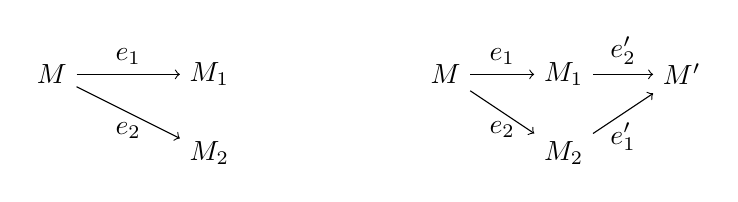
\begin{tikzpicture} %[scale=0.8]
    \node (m2) at (0,0) {\(M_2\)};
    \node (m1) at (0,1) {\(M_1\)};
    \node (m) at (-2,1) {\(M\)};
    \node (implies) at (2,1) {\(\implies\)};
    \node (mm2) at (4.5,0) {\(M_2\)};
    \node (mm1) at (4.5,1) {\(M_1\)};
    \node (n) at (6,1) {\(M'\)};
    \node (mm) at (3,1) {\(M\)};
    \draw [->] (m) -- node [left,above] {\(e_1\)} (m1);
    \draw [->] (m) -- node [left,below] {\(e_2\)} (m2);
    \draw [->] (mm) -- node [left,above] {\(e_1\)} (mm1);
    \draw [->] (mm) -- node [left,below] {\(e_2\)} (mm2);
    \draw [->] (mm1) -- node [left,above] {\(e_2'\)} (n);
    \draw [->] (mm2) -- node [left,below] {\(e_1'\)} (n);
  \end{tikzpicture}
  \]
  Moreover, for any graph $M''$ such that $M''\emb M_1$ then $M''\emb M'$.
  \item if the two productions are co-final, i.e. $M_1'\iso M_2'$ then there exists $M'$ such that the diagram commutes
  \[
  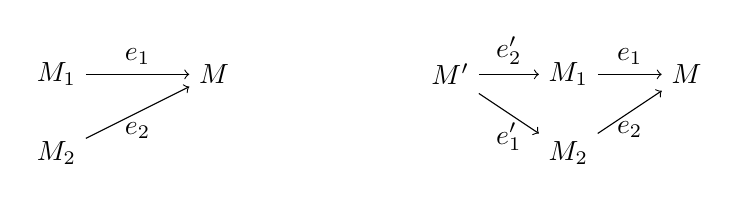
\begin{tikzpicture} %[scale=0.8]
    \node (m2) at (-2,0) {\(M_2\)};
    \node (m1) at (-2,1) {\(M_1\)};
    \node (m) at (0,1) {\(M\)};
    \node (implies) at (2,1) {\(\implies\)};
    \node (mm2) at (4.5,0) {\(M_2\)};
    \node (mm1) at (4.5,1) {\(M_1\)};
    \node (n) at (3,1) {\(M'\)};
    \node (mm) at (6,1) {\(M\)};
    \draw [->] (m1) -- node [left,above] {\(e_1\)} (m);
    \draw [->] (m2) -- node [left,below] {\(e_2\)} (m);
    \draw [->] (mm1) -- node [left,above] {\(e_1\)} (mm);
    \draw [->] (mm2) -- node [left,below] {\(e_2\)} (mm);
    \draw [->] (n) -- node [left,above] {\(e_2'\)} (mm1);
    \draw [->] (n) -- node [left,below] {\(e_1'\)} (mm2);
  \end{tikzpicture}
  \]
  Moreover, for any graph $M''$ such that $M''\emb M_1$ then $M''\emb M'$.
  \end{enumerate}
\end{lemma}

%% \begin{lemma}
%%   \label{lem:rewrite_concurrent}
%%   Let $(E,\subseteq,\labl, \bp) $ be the refinement of a decorated poset and let $e_1,e_2\in E$ be two incomparable events such that
%%   $\bp(e_1) = M_1\overset{e_1}{\Rightarrow} M_1'$ and $\bp(e_2) = M_2\overset{e_2}{\Rightarrow} M_2'$.
%%   \begin{enumerate}
%%   \item if the two productions are co-initial, i.e. $M_1\iso M_2$ then there exists $M'$ such that the diagram commutes
%%   \[
%%   \begin{tikzpicture} %[scale=0.8]
%%     \node (m2) at (0,0) {\(\circ\)};
%%     \node (m1) at (0,1) {\(\circ\)};
%%     \node (m) at (-2,1) {\(M\)};
%%     \node (implies) at (2,1) {\(\implies\)};
%%     \node (mm2) at (4.5,0) {\(\circ\)};
%%     \node (mm1) at (4.5,1) {\(\circ\)};
%%     \node (n) at (6,1) {\(M'\)};
%%     \node (mm) at (3,1) {\(M\)};
%%     \draw [->] (m) -- node [left,above] {\(e_1\)} (m1);
%%     \draw [->] (m) -- node [left,below] {\(e_2\)} (m2);
%%     \draw [->] (mm) -- node [left,above] {\(e_1\)} (mm1);
%%     \draw [->] (mm) -- node [left,below] {\(e_2\)} (mm2);
%%     \draw [->] (mm1) -- node [left,above] {\(e_2'\)} (n);
%%     \draw [->] (mm2) -- node [left,below] {\(e_1'\)} (n);
%%   \end{tikzpicture}
%%   \]
%%   \item if the two productions are co-final, i.e. $M_1'\iso M_2'$ then there exists $M'$ such that the diagram commutes
%%   \[
%%   \begin{tikzpicture} %[scale=0.8]
%%     \node (m2) at (-2,0) {\(\circ\)};
%%     \node (m1) at (-2,1) {\(\circ\)};
%%     \node (m) at (0,1) {\(M\)};
%%     \node (implies) at (2,1) {\(\implies\)};
%%     \node (mm2) at (4.5,0) {\(\circ\)};
%%     \node (mm1) at (4.5,1) {\(\circ\)};
%%     \node (n) at (3,1) {\(M'\)};
%%     \node (mm) at (6,1) {\(M\)};
%%     \draw [->] (m1) -- node [left,above] {\(e_1\)} (m);
%%     \draw [->] (m2) -- node [left,below] {\(e_2\)} (m);
%%     \draw [->] (mm1) -- node [left,above] {\(e_1\)} (mm);
%%     \draw [->] (mm2) -- node [left,below] {\(e_2\)} (mm);
%%     \draw [->] (n) -- node [left,above] {\(e_2'\)} (mm1);
%%     \draw [->] (n) -- node [left,below] {\(e_1'\)} (mm2);
%%   \end{tikzpicture}
%%   \]
%%   \end{enumerate}
%% \end{lemma}
\begin{proof}
  \begin{enumerate}
  \item Let $\labl(e_1)=L_1\action R_1$ and $\labl(e_2)=L_2\action R_2$ be the labels of the two events.
    Then there exists an event $e_3$ such that $e_3\subseteq_{O_1} e_1$ and $e_3\subseteq_{O_2} e_2$. We can assume without loss of generality, that $e_3$ is the only such event (in the cover relation with $e_1$ and $e_2$). Let us show that we can rewrite $M_1'$ using rule $\labl(e_2)$ and obtain $M'$ such that $M_1\overset{e_1}{\Rightarrow} M_1'$ and $M_1'\overset{e_2'}{\Rightarrow} M_2'$ are sequentially independent.

     Let us consider only the poset restricted to events $\{e_1,e_2,e_3\}$. We have that, in the following diagram, there exists a morphism $L_2\to D'$ that commutes.
     \[
     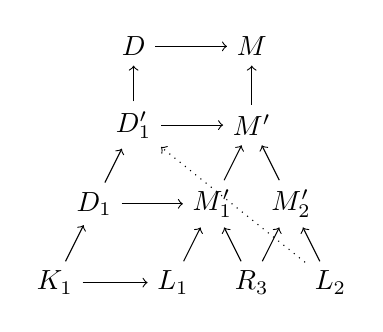
\begin{tikzpicture} %[scale=0.8]
       \node (k1) at (0,0) {\(K_1\)};
       \node (l1) at (1.5,0) {\(L_1\)};
       \node (r3) at (2.5,0) {\(R_3\)};
       \node (l2) at (3.5,0) {\(L_2\)};
       \node (m1) at (2,1) {\(M_1'\)};
       \node (m2) at (3,1) {\(M_2'\)};
       \node (d1) at (0.5,1) {\(D_1\)};
       \node (d1p) at (1,2) {\(D_1'\)};
       \node (m1p) at (2.5,2) {\(M'\)};
       \node (d) at (1,3) {\(D\)};
       \node (m) at (2.5,3) {\(M\)};
       \draw [->] (k1) -- (l1);
       \draw [->] (k1) -- (d1);
       \draw [->] (d1) -- (d1p);
       \draw [->] (d1) -- (m1);
       \draw [->] (d1p) -- (d);
       \draw [->] (d1p) -- (m1p);
       \draw [->] (d) -- (m);
       \draw [->] (l1) -- (m1);
       \draw [->] (r3) -- (m1);
       \draw [->] (r3) -- (m2);
       \draw [->] (l2) -- (m2);
       \draw [->] (m2) -- (m1p);
       \draw [->] (m1) -- (m1p);
       \draw [->] (m1p) -- (m);
       \draw [dotted,->] (l2) -- (d1p);
     \end{tikzpicture}
     \]

     Using the corollar of~\autoref{lem:subposet} if there is no such morphism then events are sequential dependent in the original trace. From~\autoref{def:abstraction}, one has that $e_1 < e_2$, which contradicts the hypothesis.

     If there exists a morphism $L_2\to D'$ that commutes then, using~\autoref{lem:subposet} there is a morphism from $L_2\to D$ that commutes.
     Lastly we use~\autoref{church_rosser} which from such a morphism, infers that $M\overset{e_1}{\Rightarrow} M_1'$ and $M\overset{e_2}{\Rightarrow} M_2'$ are parallel independent.

  \item As we are using DPO rewriting, this case is similar to the first.
  \end{enumerate}
\end{proof}


\begin{definition}[Concretisation of a poset]
  \label{def:concretisation}
  Given a set of posets $\mathcal{S}$ let us define the concretisation function $\gamma:\mathcal{S}\subseteq\Theta$ that sends a poset to a set of traces.
  \begin{itemize}
  \item For $s\in\mathcal{S}$, let $\overline{s}\in\decor(s)$ be a decorated poset.
    We define the refinement of a decorated poset $\mathit{refine}(\overline{s}) = \{E,\sqsubset,\labl,\bp\}$, where $\overline{s} = \{E,\sqsubset,\labl\}$.
  \item For every pair of concurrent events in $\mathit{refine}(\overline{s})$ close out the diagram using~\autoref{lem:rewrite_concurrent}. Denote $S$ a diagram that is closed with respect to the concurrent events. Then define $\gamma$, the concretisation function, as a set of traces, where each trace is a path in the diagram $S$:
    \[
    \gamma(s) = \{ t : t\text{ is a path in }S\text{ and }S\text{ is one the closed diagrams of }\mathit{refine}(\decor(s))\}.
    \]
  \end{itemize}
\end{definition}

\begin{example}
  We complete the refined poset of the left by applying~\autoref{lem:rewrite_concurrent} to obtain the diagram on the right:
  \[
  \begin{tikzpicture} %[scale=0.8]
  \node (n2) at (-1,1) {\(\circ\)};
  \node (m2) at (0,0) {\(\circ\)};
  \node (m1) at (0,1) {\(\circ\)};
  \node (n) at (1,1) {\(\circ\)};
  \node (implies) at (2,1) {\(\leadsto\)};
  \node (mm2) at (5.6,0) {\(\circ\)};
  \node (mm1) at (5.6,1) {\(\circ\)};
  \node (nn) at (6.9,1) {\(\circ\)};
  \node (mm) at (4.3,0) {\(\circ\)};
  \node (nn1) at (3,0) {\(\circ\)};
  \node (nn2) at (4.3,1) {\(\circ\)};
  \node (text) at (0.8,0.4) {\(e_3\)};
  \node (text1) at (5.3,0.5) {\(e_3'\)};
  \draw [->] (n2) -- node [left,above] {\(e_1\)} (m1);
  \draw [->] (m1) -- node [left,above] {\(e_2\)} (n);
  \draw [->] (m2) -- (n);
  \draw [->] (nn2) -- node [left,above] {\(e_1\)} (mm1);
  \draw [->] (mm1) -- node [left,above] {\(e_2\)} (nn);
  \draw [->] (mm2) -- node [left,below] {\(e_3\)} (nn);
  \draw [->] (mm) -- node [left,below] {\(e_2'\)} (mm2);
  \draw [->] (mm) -- (mm1);
  \draw [->] (nn1) -- node [above] {\(e_3''\)} (nn2);
  \draw [->] (nn1) -- node [left,below] {\(e_1'\)} (mm);
\end{tikzpicture}
\]
\end{example}

%% \[
%% \begin{tikzpicture} %[scale=0.8]
%%   \node (m2) at (0,0) {\(\circ\)};
%%   \node (m1) at (0,1) {\(\circ\)};
%%   \node (n) at (1,1) {\(\circ\)};
%%   \node (n1) at (2,1) {\(\circ\)};
%%   \node (n2) at (2,0) {\(\circ\)};
%%   \node (implies) at (3,1) {\(\leadsto\)};
%%   \node (m) at (4,1) {\(\circ\)};
%%   \node (mm2) at (5,0) {\(\circ\)};
%%   \node (mm1) at (5,1) {\(\circ\)};
%%   \node (nn) at (6,1) {\(\circ\)};
%%   \node (nn1) at (7,1) {\(\circ\)};
%%   \node (nn2) at (7,0) {\(\circ\)};
%%   \node (p) at (8,1) {\(\circ\)};
%%   \draw [->] (n) -- node [left,above] {\(e_3\)} (n1);
%%   \draw [->] (n) -- node [left,below] {\(e_4\)} (n2);
%%   \draw [->] (m1) -- node [left,above] {\(e_1\)} (n);
%%   \draw [->] (m2) -- node [left,below] {\(e_2\)} (n);
%%   \draw [->] (nn) -- node [left,above] {\(e_3\)} (nn1);
%%   \draw [->] (nn) -- node [left,below] {\(e_4\)} (nn2);
%%   \draw [->] (mm1) -- node [left,above] {\(e_1\)} (nn);
%%   \draw [->] (mm2) -- node [left,below] {\(e_2\)} (nn);
%%   \draw [->] (m) -- node [left,above] {\(e_2'\)} (mm1);
%%   \draw [->] (m) -- node [left,below] {\(e_1'\)} (mm2);
%%   \draw [->] (nn1) -- node [left,above] {\(e_3'\)} (p);
%%   \draw [->] (nn2) -- node [left,below] {\(e_4'\)} (p);
%% \end{tikzpicture}
%% \]
%% \[
%% \begin{tikzpicture} %[scale=0.8]
%%   \node (m) at (-1,1) {\(\circ\)};
%%   \node (m2) at (0,0) {\(\circ\)};
%%   \node (m1) at (0,1) {\(\circ\)};
%%   \node (n) at (1,1) {\(\circ\)};
%%   \node (implies) at (2,1) {\(\leadsto\)};
%%   \node (implies2) at (7,1) {\(~\)};
%%   \draw [->] (m) -- node [left,above] {\(e_1\)} (m1);
%%   \draw [->] (m) -- node [left,below] {\(e_2\)} (m2);
%%   \draw [->] (m1) -- node [left,above] {\(e_3\)} (n);
%%   \draw [->] (m2) -- node [left,below] {\(e_4\)} (n);
%% \end{tikzpicture}
%% \]

\begin{lemma}
  $\theta\subseteq \gamma(\alpha(\theta))$.
\end{lemma}
\begin{proof}
    \begin{mdframed}[backgroundcolor=blue!20]
    to do
  \end{mdframed}
\end{proof}

\begin{remark}[Adding inhibition]
  We can change definition~\autoref{def:abstraction} in order to construct posets with the additional relation of inhibition between events:
  \[
  e_i \dashv e_j \iff t_i \dashv t_j \text{ and } \alpha(t_i)=e_i, \alpha(t_j)=e_j
  \]
  Inhibition doesn't change the decoration and refinement of a poset but can make the concretisation function "more precise". In~\autoref{def:concretisation} we have to additionally remove any path in $\gamma(\alpha(\theta))$ that has two events $e_1$ followed by $e_2$ such that $e_1\dashv e_2$.
\end{remark}
